\subsection{Hierarchical clustering}

In report 2, we found that the classification method K-nearest neighbours with the distance measure \textcolor{Bittersweet}{\textit{correlation}} yielded the best results for classification, so we will use the dissimilarity measure \textcolor{Bittersweet}{\textit{correlation}}. We tried hierarchical clustering with several different linkage functions (single/minimum, complete/maximum, ward). The focus for plots will be at the cut-off at 7 clusters.

\begin{multicols}{2}
\begin{figure}[H]
    \centering
    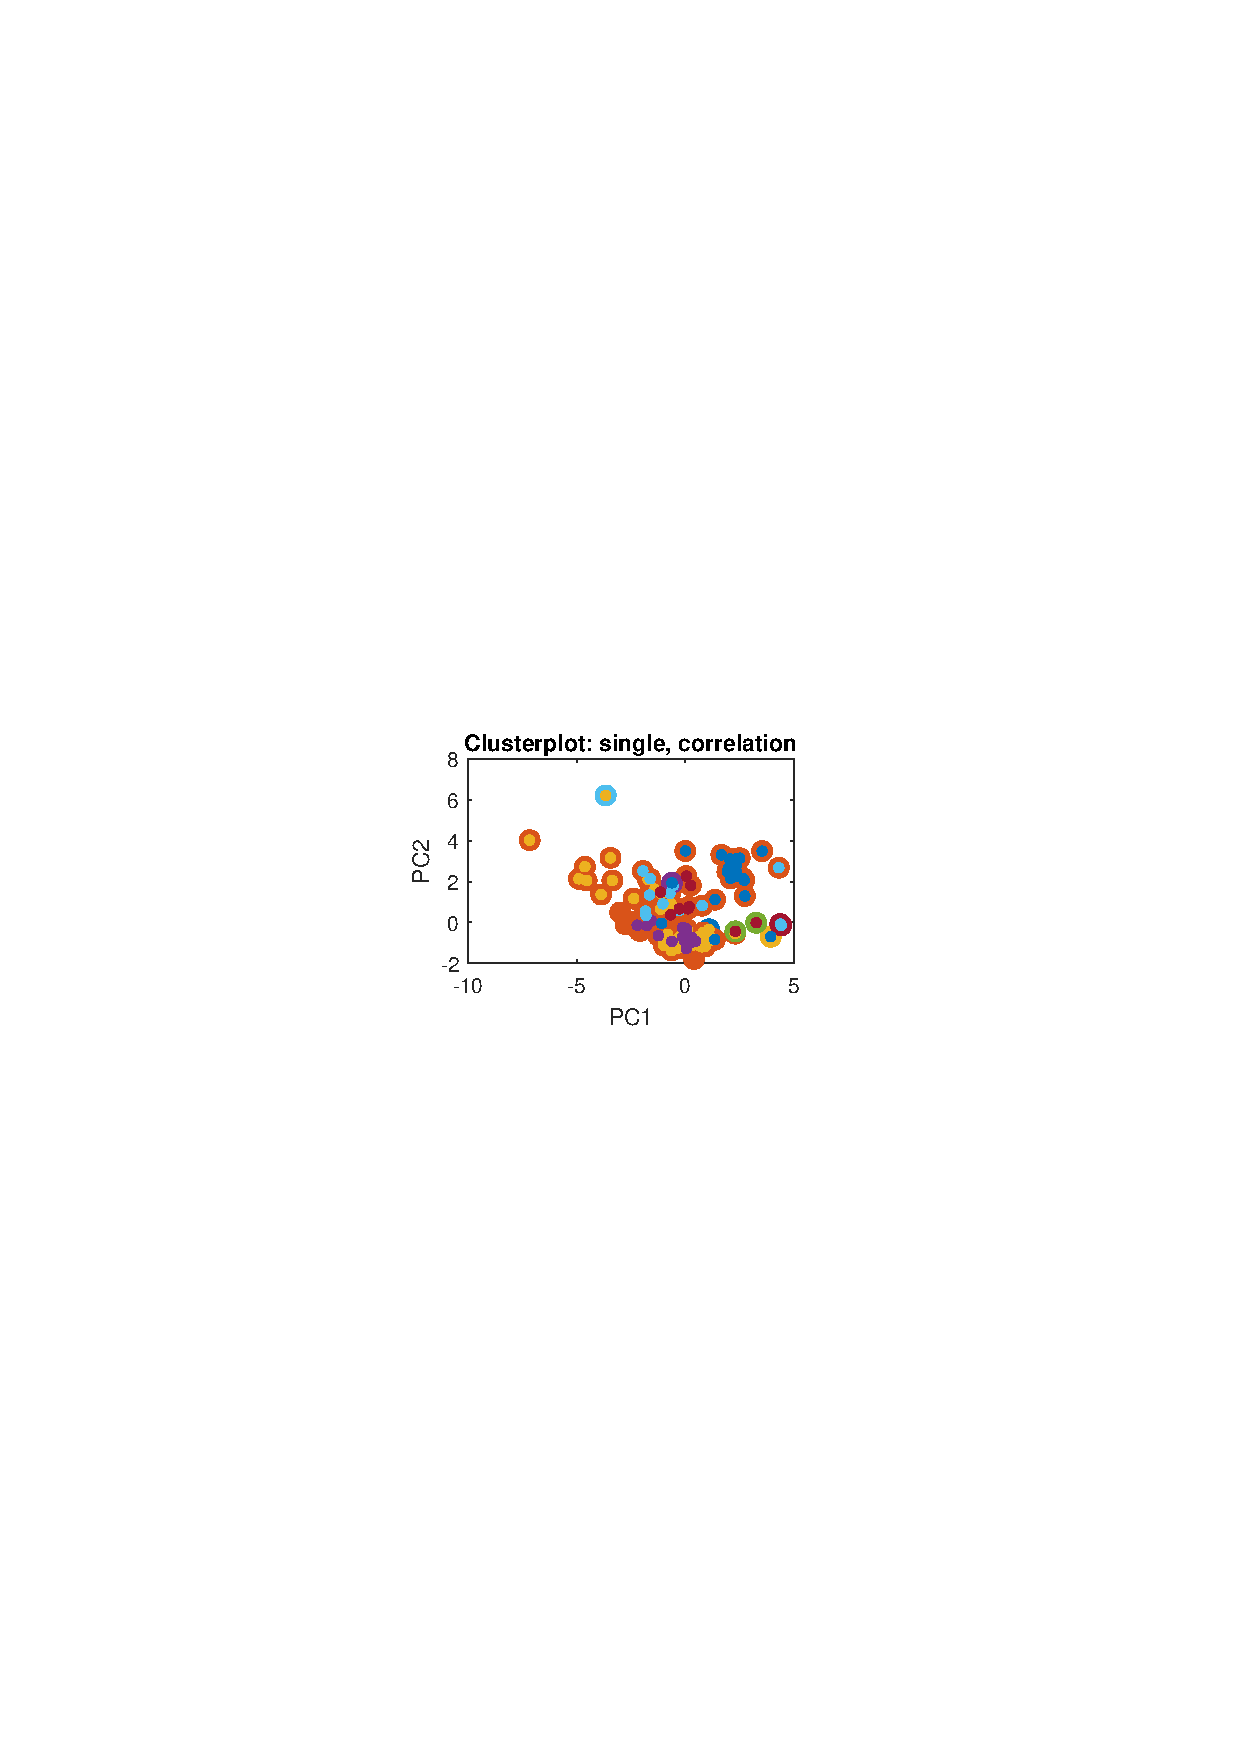
\includegraphics[width=0.4\textwidth]{fig/cluster_single_cor.pdf}
    \caption{7 clusters based on hierarchical clustering with minimum/single linkage and correlation as dissimilarity measure.}
    \label{fig:cluster_single_cor}
\end{figure}

\begin{figure}[H]
    \centering
    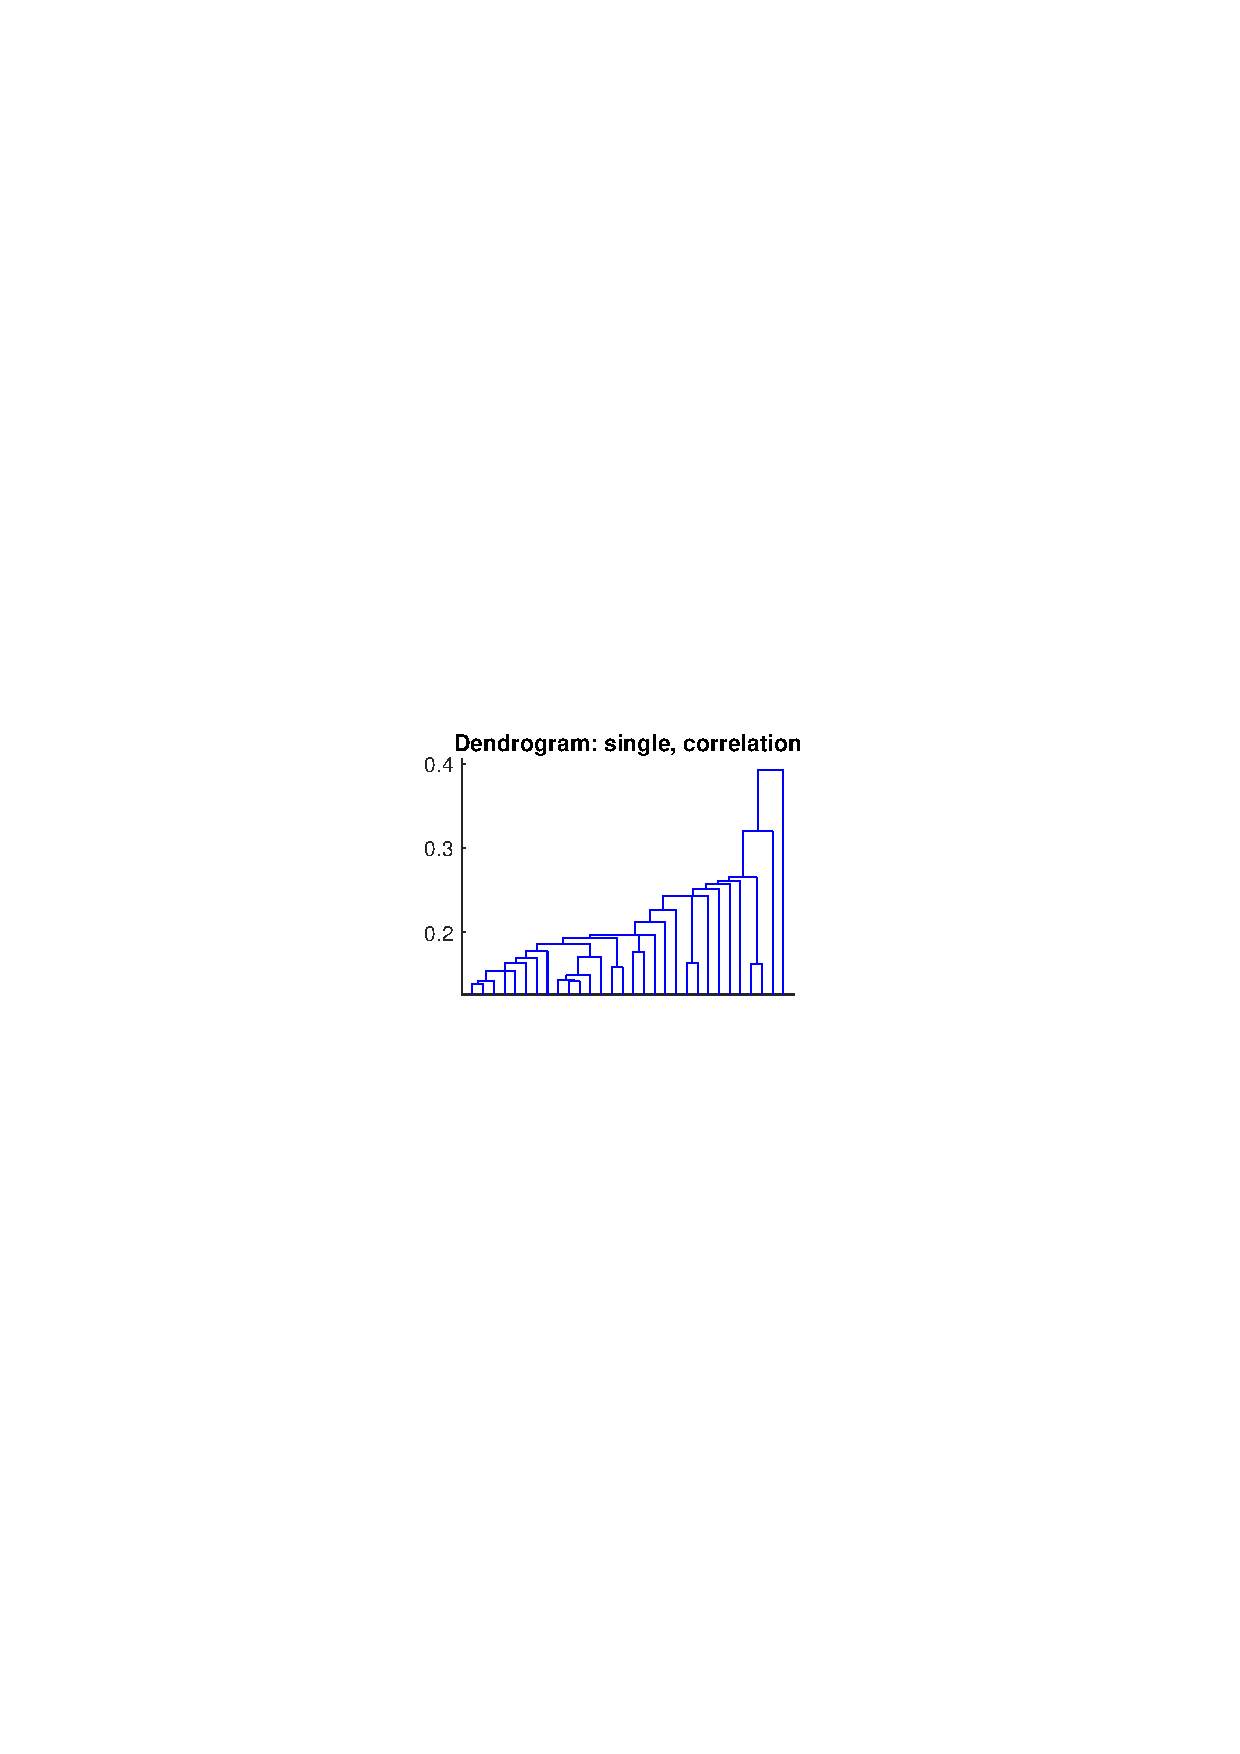
\includegraphics[width=0.4\textwidth]{fig/dendro_single_cor.pdf}
    \caption{Dendrogram for the hierarchical clustering with minimum/single linkage and correlation as dissimilarity measure.}
    \label{fig:dendro_single_cor}
\end{figure}

\end{multicols}


\begin{multicols}{2}
\begin{figure}[H]
    \centering
    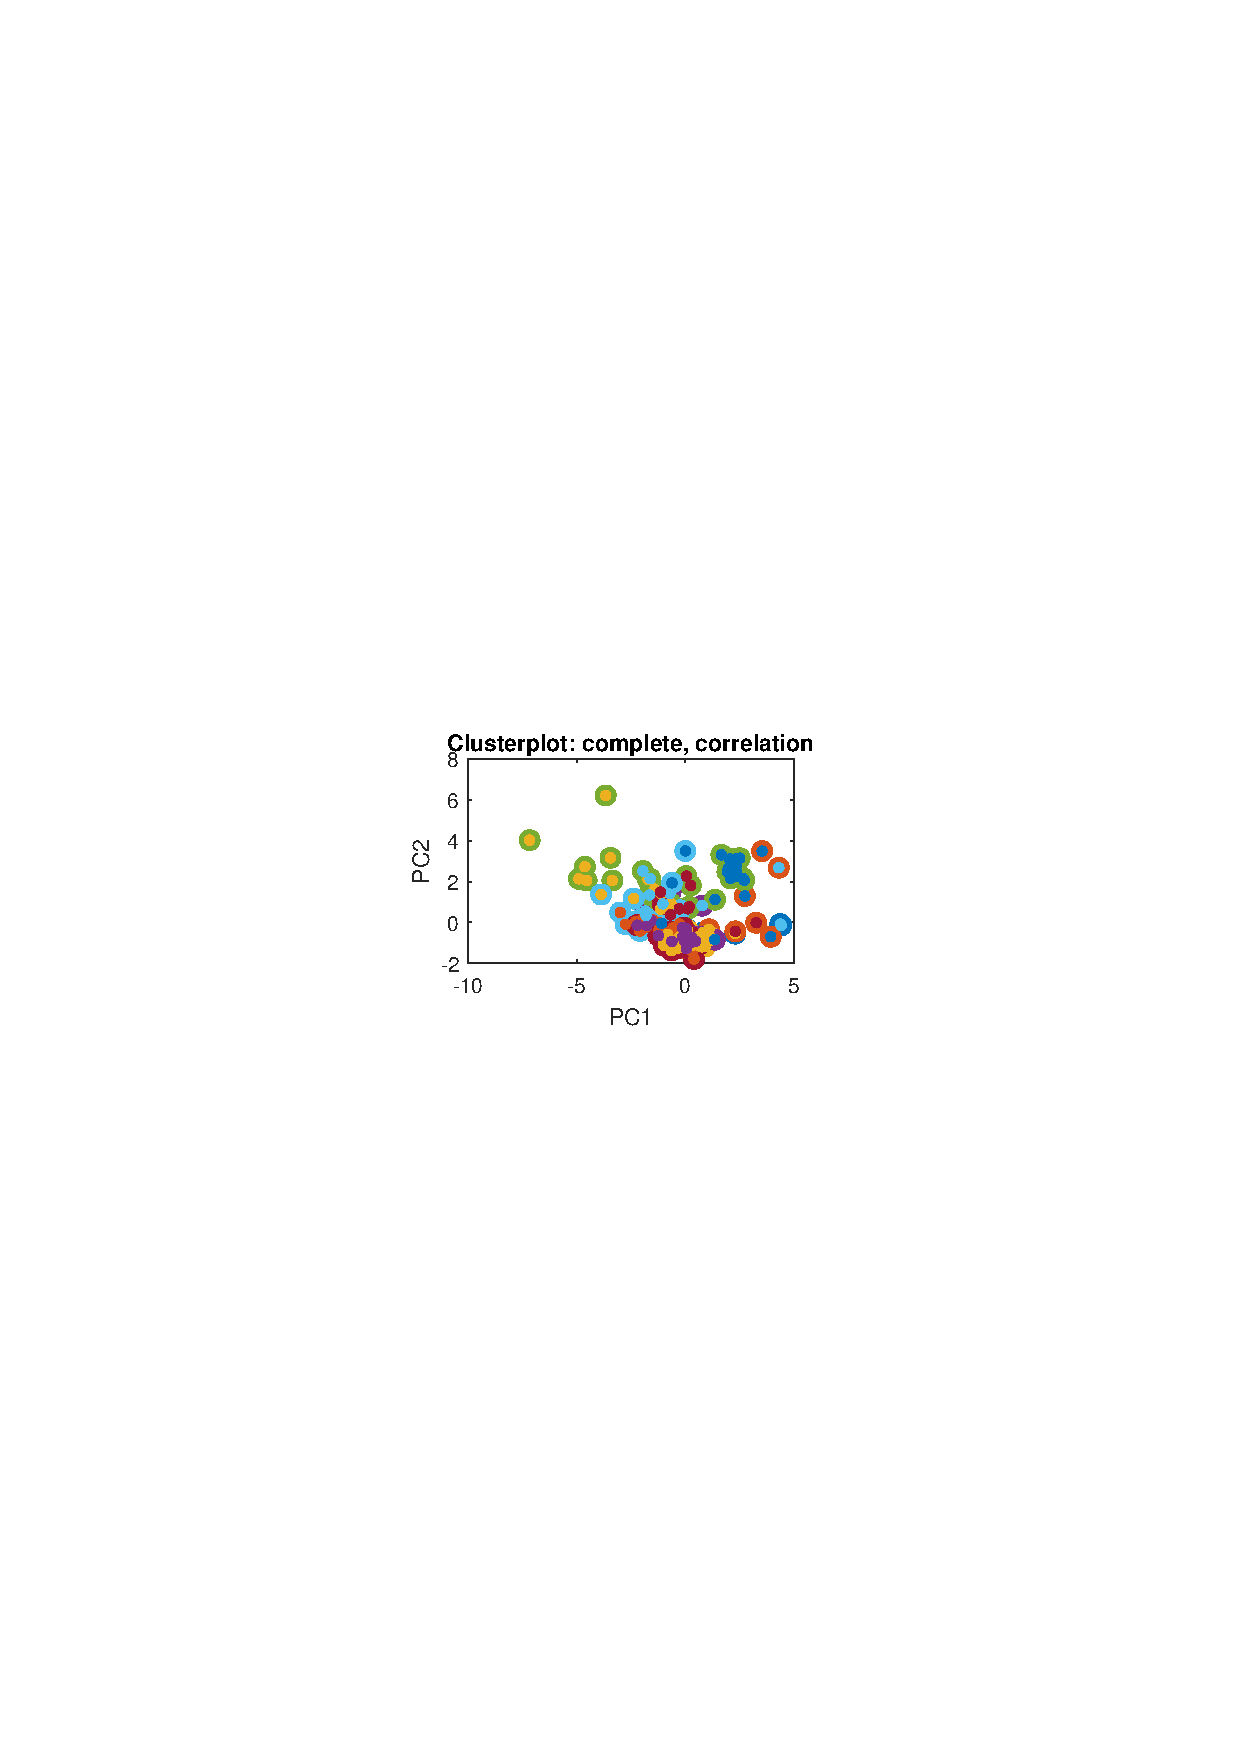
\includegraphics[width=0.4\textwidth]{fig/cluster_complete_cor.pdf}
    \caption{7 clusters based on hierarchical clustering with maximum/complete linkage and correlation as dissimilarity measure.}
    \label{fig:cluster_complete_cor}
\end{figure}

\begin{figure}[H]
    \centering
    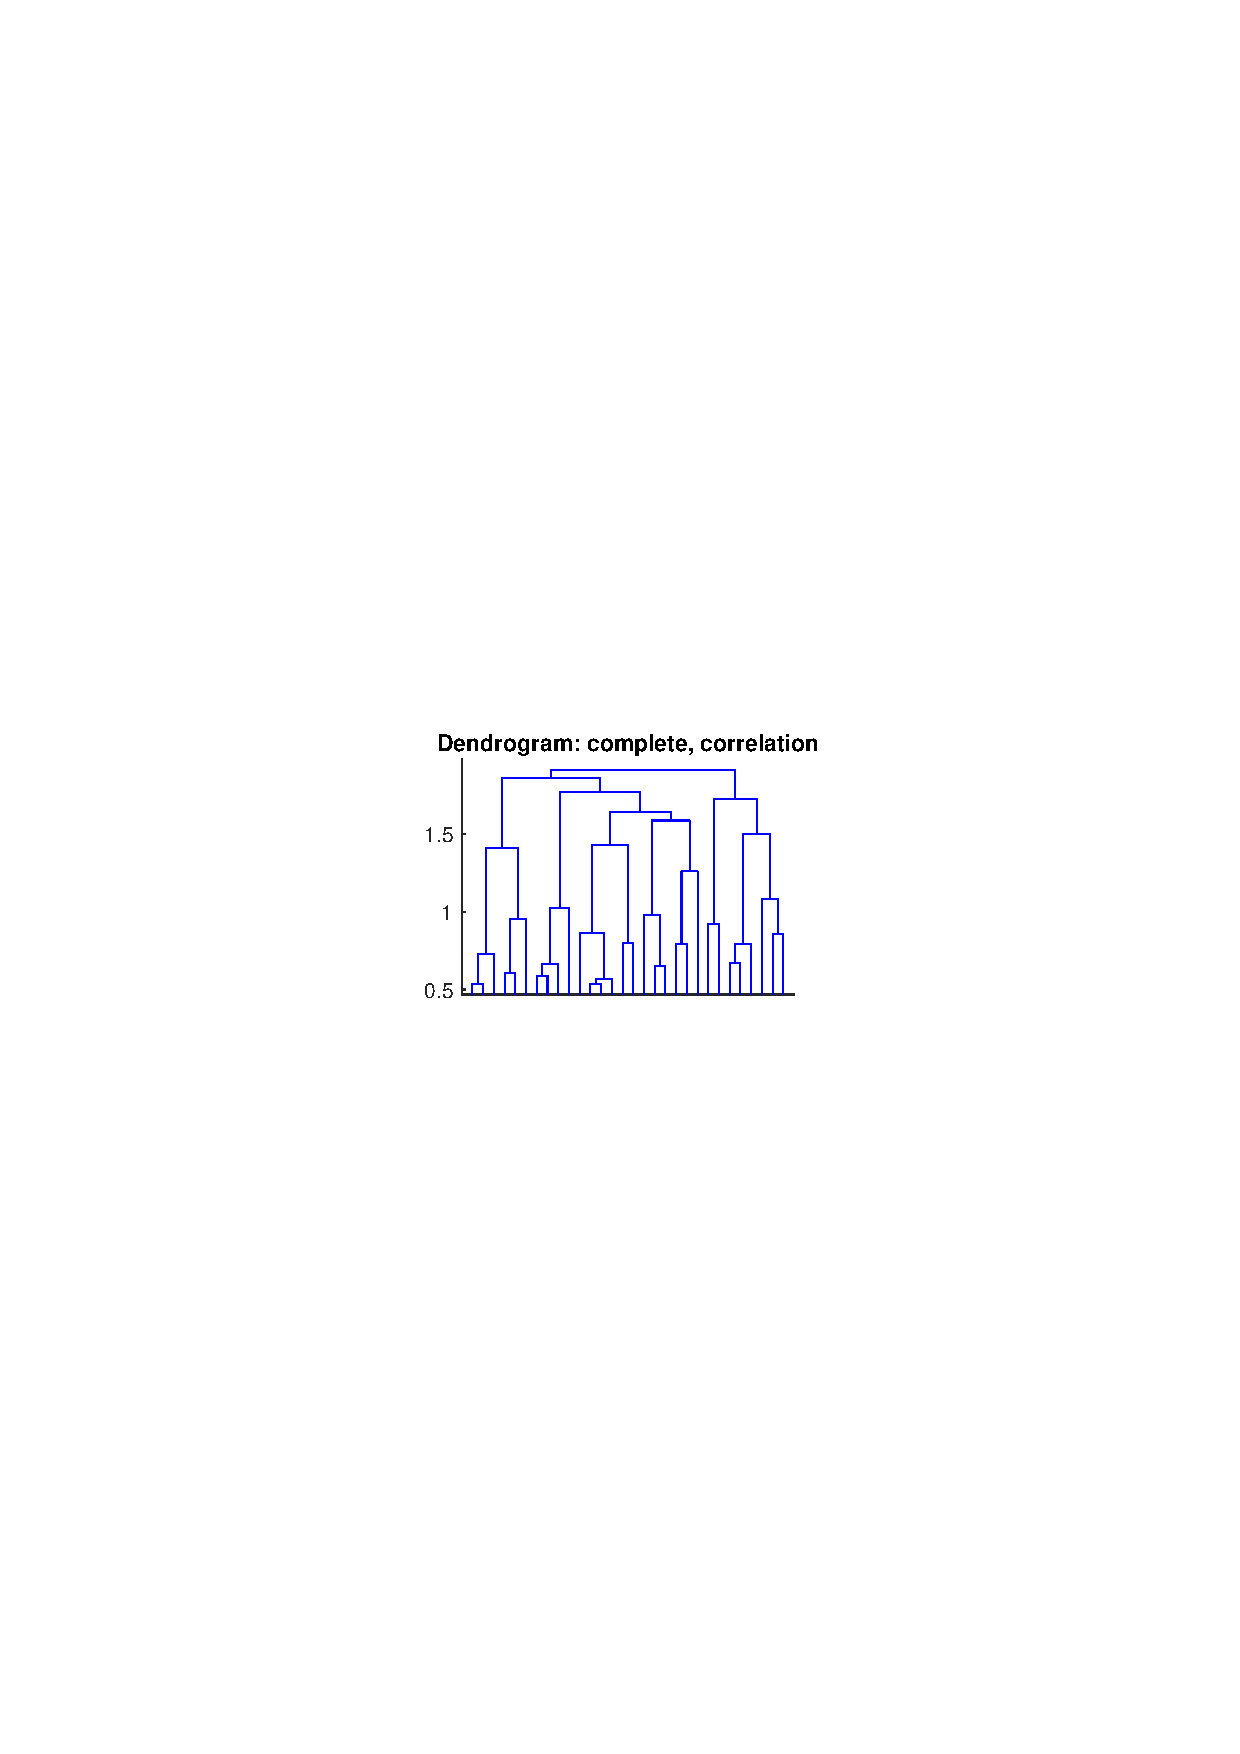
\includegraphics[width=0.4\textwidth]{fig/dendro_complete_cor.pdf}
    \caption{Dendrogram for the hierarchical clustering with maximum/complete linkage and correlation as dissimilarity measure.}
    \label{fig:dendro_complete_cor}
\end{figure}

\end{multicols}

\begin{multicols}{2}
\begin{figure}[H]
    \centering
    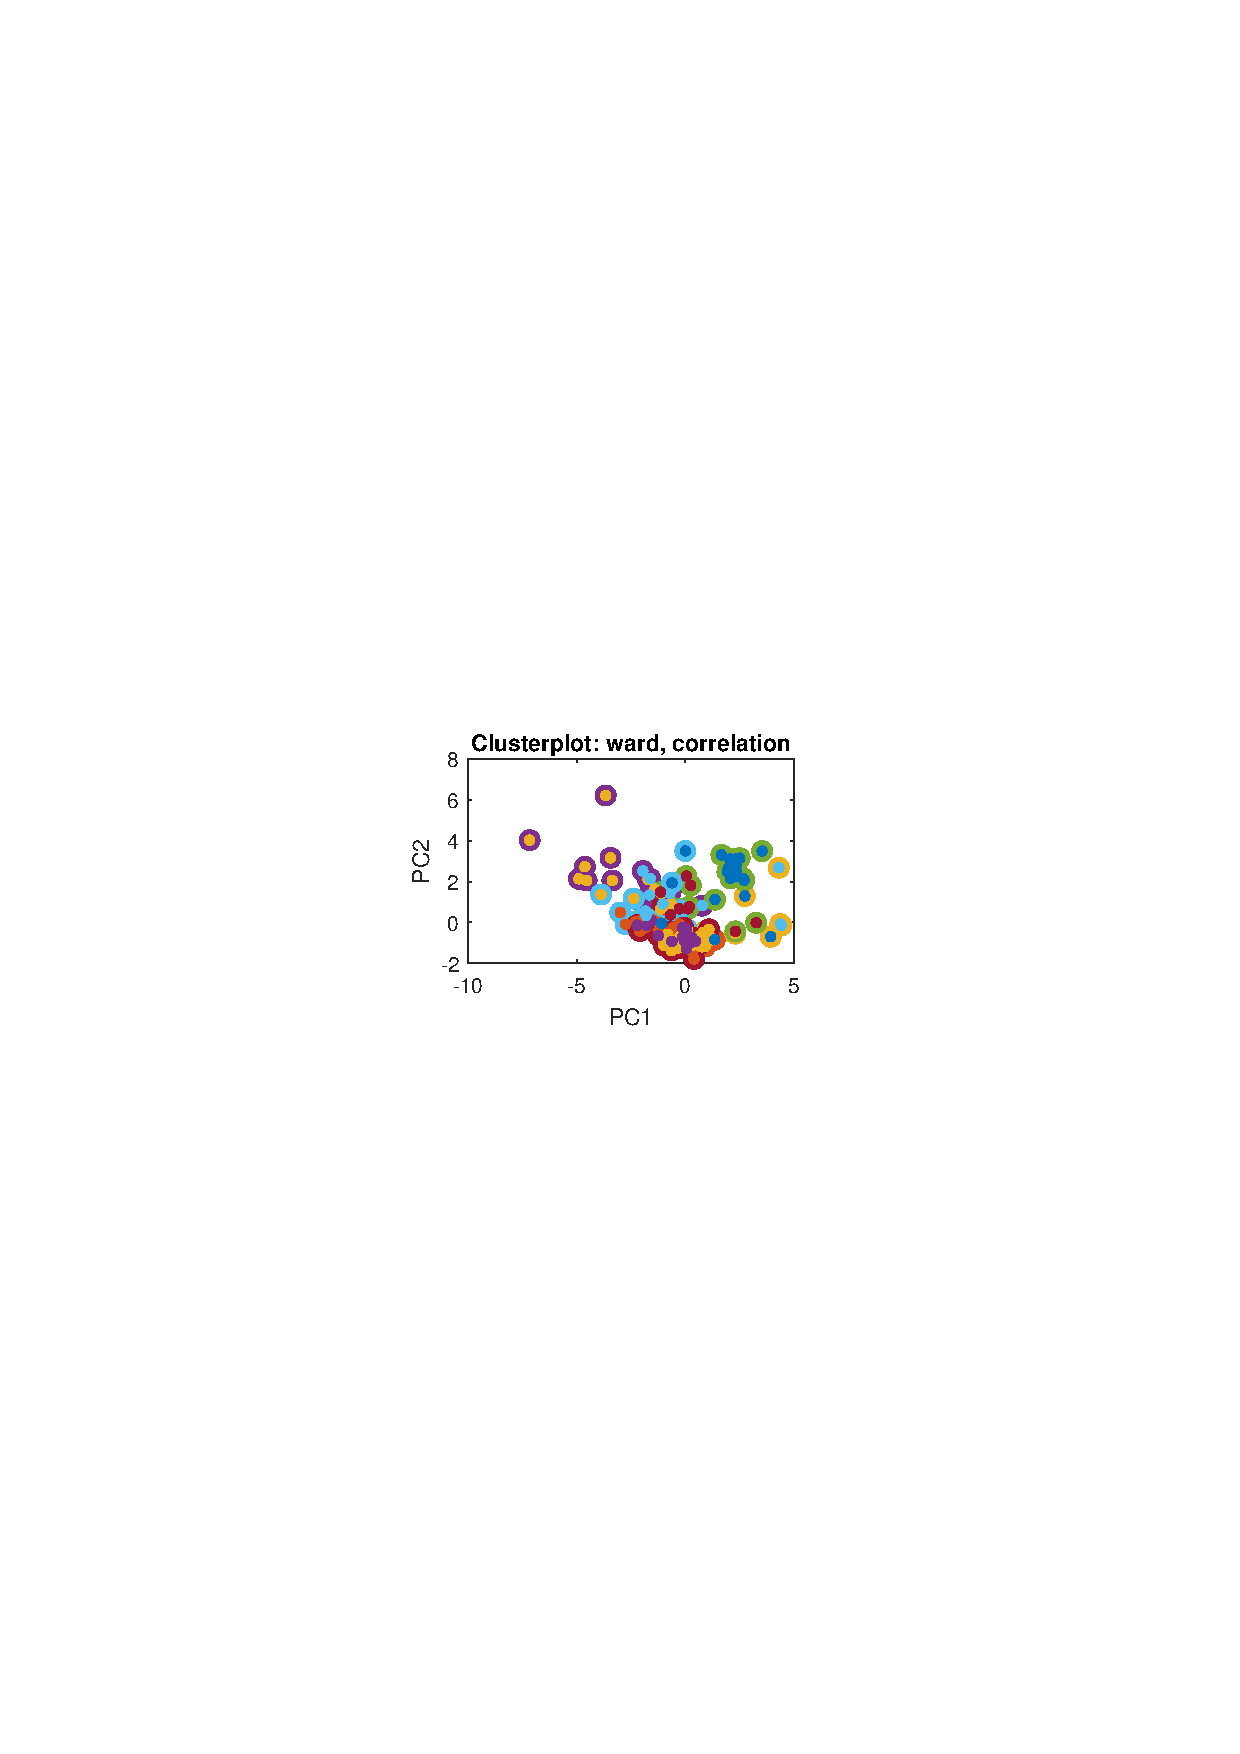
\includegraphics[width=0.4\textwidth]{fig/cluster_ward_cor.pdf}
    \caption{7 clusters based on hierarchical clustering with ward linkage and correlation as dissimilarity measure.}
    \label{fig:cluster_ward_cor}
\end{figure}

\begin{figure}[H]
    \centering
    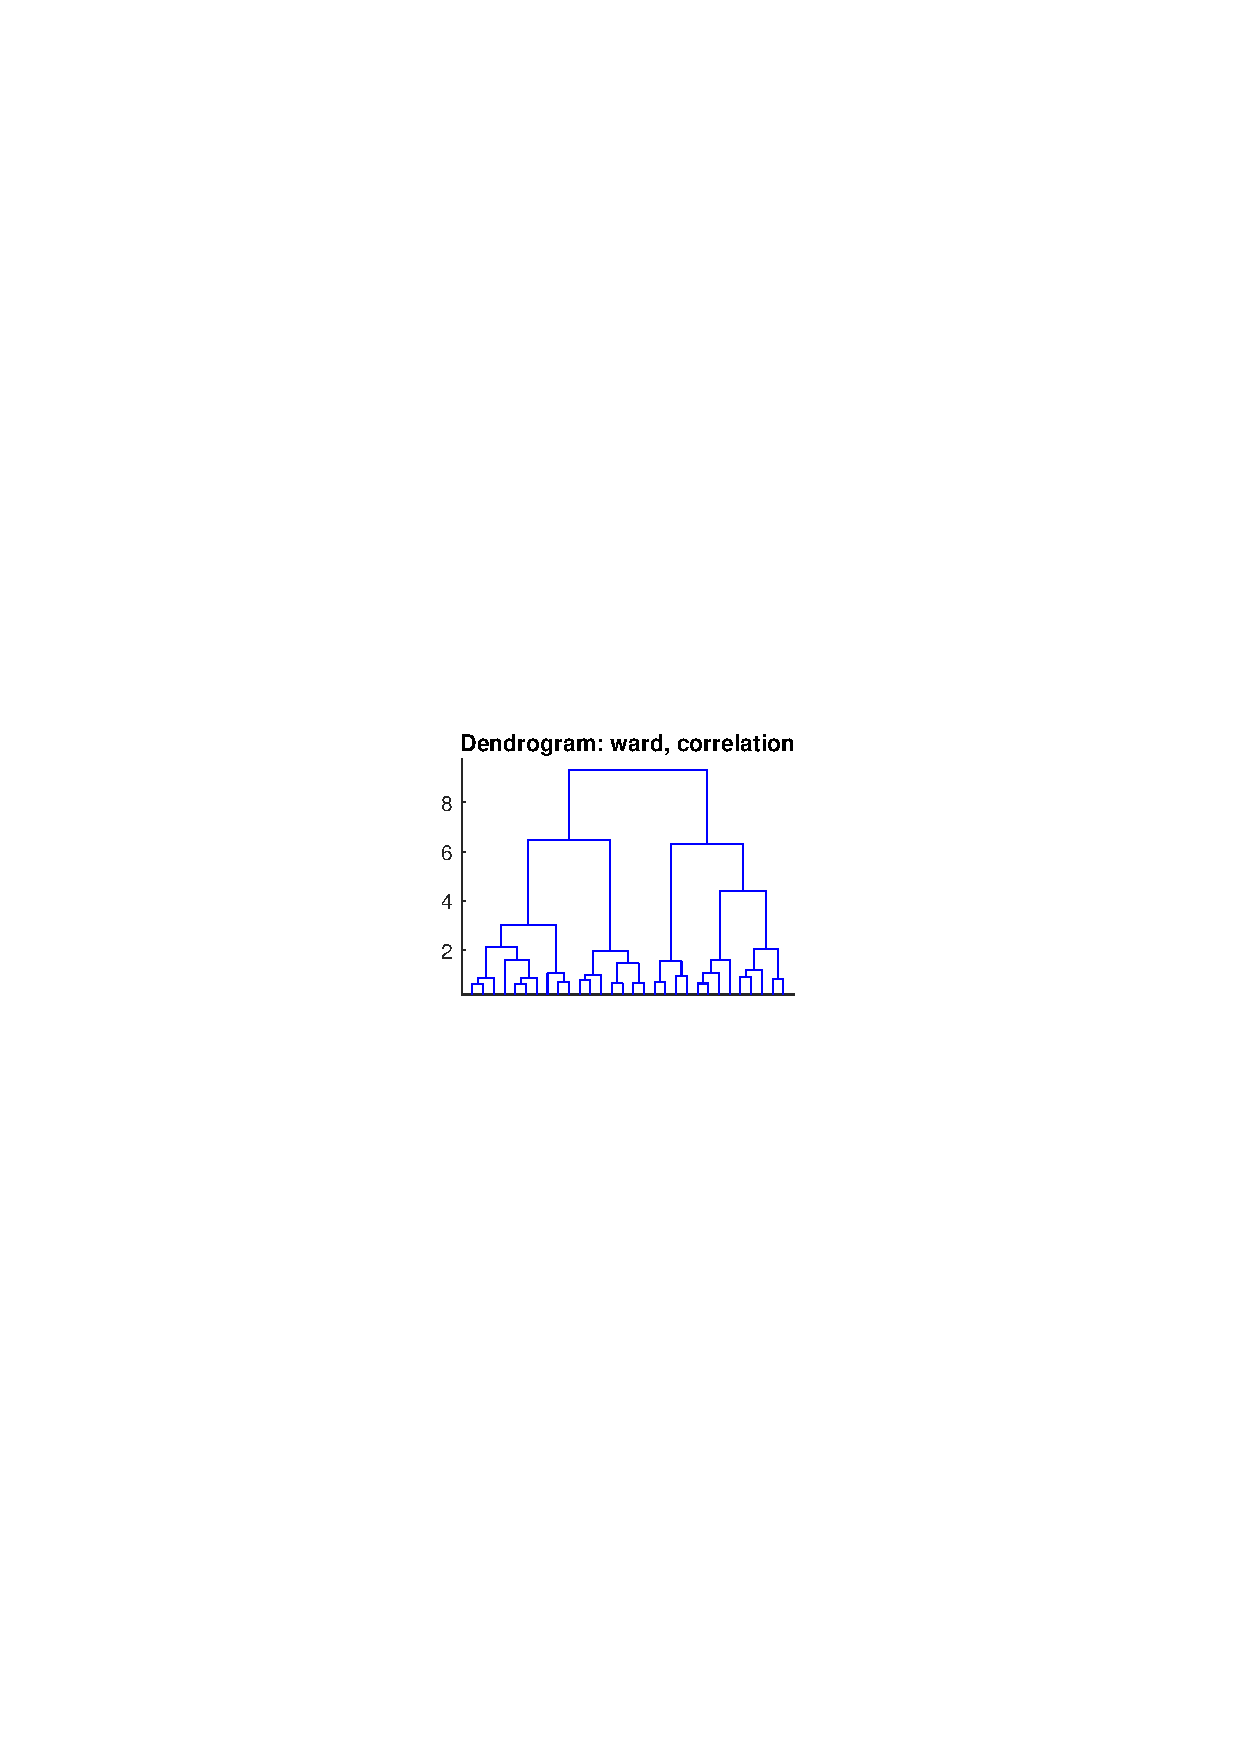
\includegraphics[width=0.4\textwidth]{fig/dendro_ward_cor.pdf}
    \caption{Dendrogram for the hierarchical clustering with ward linkage and correlation as dissimilarity measure.}
    \label{fig:dendro_ward_cor}
\end{figure}

\end{multicols}
